\scanpage{70}\mspage{69}
J'en viens à la rel d'ordre $\preceq$ (subdivision), de nature \unsure{très|trs} différente. Il n'y \unsure{aura} pas de plus petit (ni de plus grand) élément, pas de $\mathrm{Sup}$ de deux \deleted{\unsure{éléments|élémen}}
% G1: local interlinear layout; the separate oblique arm has no supplied arrowhead.
\figure{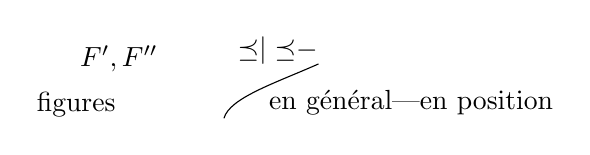
\begin{tikzpicture}[x=1cm,y=1cm]
\node[anchor=base west] at (0,0) {figures};
\node[anchor=base west] at (0.55,0.58) {\inserted{$F',F''$}};
\node[anchor=base west] at (2.55,0.69) {$\inserted{\unsure{\deleted{\preceq}|\preceq}-}$};
\draw (2.50,-0.08) .. controls (2.57,0.18) and (3.16,0.37) .. (3.70,0.61);
\node[anchor=base west] at (2.95,0.03) {\unsure{en général|en position}};
\end{tikzpicture}}
(i.e. Subdivisions d'une $=$ figure $F$, mais parfois un $\inf$.

On dit que deux subdivision $F',F'''$ de $F$ sont \uline{comp\deleted{\unsure{ati|atib}}\unsure{ara|ati|ata}bles} \deleted{\unsure{quand et|on dit|c.à.d.} que \unsure{seulement|sub}} (je ne dirai pas ``compatibles'', vu que le terme est déjà pris) si elles admettent une subdivision commune.

% D1: the sole right F is level with the upper F'; the lower-right relation ends in blank space.
% The additional thin upper stroke belongs to the worked upper-right relation; no separate complete older glyph is asserted.
\diagram{\begin{tikzcd}[ampersand replacement=\&,row sep=0.25em,column sep=0.4em]
\& F' \arrow[r,phantom,"{\begin{tikzpicture}[baseline=-0.5ex,x=0.5cm,y=0.5cm]\node at (0,0) {$\scriptstyle\unsure{\preceq}$};\draw[thin] (-0.18,0.02) -- (0.24,0.28);\end{tikzpicture}}" description] \& F \\
F''' \arrow[ur,phantom,"\scriptstyle\preceq" description,sloped] \arrow[dr,phantom,"\scriptstyle\preceq" description,sloped] \& \& {} \\
\& F'' \arrow[ur,phantom,"\scriptstyle\preceq" description,sloped] \&
\end{tikzcd}}
% slanted
\margin{On sera amené à renforcer encore cette condition sur les contrées modérées !}

On dit que la \uuline{\unsure{contrée|contrie}} est \uuline{modérée} si deux subdivisions \unsure{d'|\deleted{d'}}\unsure{une|un} $=$ $F$ sont toujours comparables. \deleted{Dans le cas qui vient,}
% G3: cancelled words and their two detached points, kept without assigning punctuation function.
\figure{\begin{tikzpicture}[x=1cm,y=1cm]
\node[anchor=base west] at (0,0) {\deleted{on a}};
\fill (1.65,0.10) circle (0.012);
\fill (1.75,0.02) circle (0.012);
\end{tikzpicture}}

\deleted{\uline{C5}} Je ne saurais donner aucune propriété particulière de $\preceq$ \deleted{tout} seul. Les propriétés que j'ai en vue concernent \unsure{ses|les} relations avec $\leq$.

% slanted
\margin{Reporter après C6, $C7_0$ \unsure{ces|mes} axiomes de \uline{disjonction}}
% G4: the two long marks stand to the left of the live C5 axiom.
\figure{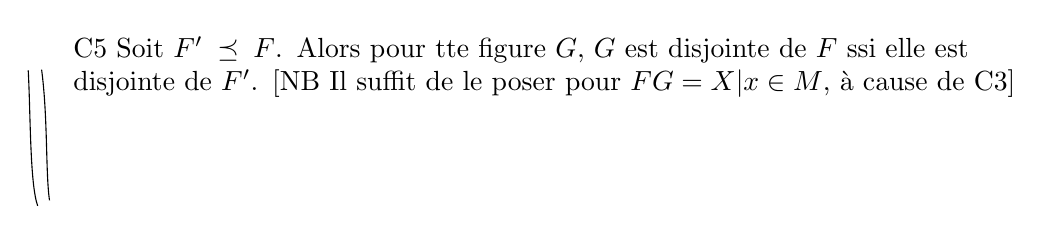
\begin{tikzpicture}[x=1cm,y=1cm]
\draw (0,0) .. controls (0.03,-0.55) and (0.02,-1.44) .. (0.12,-1.72);
\draw (0.17,0.01) .. controls (0.25,-0.60) and (0.22,-1.30) .. (0.27,-1.65);
\node[anchor=north west,text width=12cm,align=left] at (0.45,0.55) {\uline{C5} Soit $F'\preceq F$. Alors pour tte figure $G$, $G$ est disjointe de $F$ ssi elle est disjointe de $F'$. [\uline{NB} Il suffit de le poser pour $\deleted{\unsure{F}}G=\unsure{X|x}\in M$, à cause de C3]};
\end{tikzpicture}}
